\documentclass[12pt]{article}

% ---------------------------
% Packages
% ---------------------------
\usepackage[utf8]{inputenc}
\usepackage{xcolor}
\usepackage{hyperref}
\usepackage{listings}
\usepackage{booktabs}
\usepackage{geometry}
\usepackage{tcolorbox}
\usepackage{tikz}
\usepackage{graphicx} % For images
\usetikzlibrary{positioning} % For TikZ positioning
\geometry{margin=1in}

% ---------------------------
% Tickezy Color Palette
% ---------------------------
\definecolor{tickezyNavy}{HTML}{0A1F44}
\definecolor{tickezyNavyLight}{HTML}{0D2A5C}
\definecolor{tickezyCyan}{HTML}{3BC9F5}
\definecolor{tickezyGray}{HTML}{C7D2E0}

% ---------------------------
% Listings / Code Style
% ---------------------------
\lstset{
    basicstyle=\ttfamily\footnotesize\color{tickezyNavy},
    keywordstyle=\color{tickezyCyan}\bfseries,
    commentstyle=\color{tickezyGray}\itshape,
    stringstyle=\color{red},
    showstringspaces=false,
    frame=single,
    backgroundcolor=\color{white},
    breaklines=true
}

% ---------------------------
% Speaker Notes Box Style
% ---------------------------
\tcbset{
    speaker/.style={
        colback=tickezyCyan!15,
        colframe=tickezyCyan,
        coltitle=tickezyNavy,
        fonttitle=\bfseries,
        fontupper=\color{tickezyNavy},
        boxrule=0.8pt,
        arc=4pt,
        left=2mm,
        right=2mm,
        top=1mm,
        bottom=1mm
    }
}

% ---------------------------
% Title Page
% ---------------------------
\begin{document}

\begin{titlepage}
\centering
\vspace*{2cm}
{\Huge \textbf{TICKEZY}}\\[0.3cm]
{\Large \textcolor{tickezyCyan}{Event • Ticket • Moment}}\\[1cm]
{\large A Real-World Ticketing App Built with Swift \& SwiftUI}\\[1cm]
\textcolor{tickezyGray}{
UMURERWA Lisa Ornella \\ 
MUGABO André
}
\vfill
\textcolor{tickezyGray}{SwiftUI Pitch Presentation \\ \today}
\end{titlepage}

\newpage
\tableofcontents
\newpage

% ---------------------------
% Introduction
% ---------------------------
\section{Introduction}
Tickezy is a real-world iOS ticketing app built using Swift and SwiftUI.  
It focuses on **fast, smooth, and intuitive ticketing** for users.

\begin{tcolorbox}[speaker,title=Speaker Notes]
Lisa: Good morning. We are UMURERWA Lisa Ornella and MUGABO André.
Today we are presenting Tickezy, a real-world ticketing application
built using Swift and SwiftUI.
\end{tcolorbox}

\subsection{Core Message}
\begin{itemize}
    \item Demonstrates real-world iOS development using SwiftUI.
    \item Emphasizes clean, scalable, and maintainable architecture.
    \item Focus on smooth user experience and modern SwiftUI practices.
\end{itemize}

\begin{tcolorbox}[speaker,title=Speaker Notes]
Lisa: This presentation focuses on how we used SwiftUI
to build a clean, modern, and scalable iOS application.
\end{tcolorbox}

% ---------------------------
% Problem Statement
% ---------------------------
\section{Problem Statement}
\begin{itemize}
    \item Buying event tickets can be slow, confusing, or unintuitive.
    \item Users expect **native mobile apps** that are responsive and visually appealing.
\end{itemize}

\textbf{Opportunity:} Build a simple and intuitive ticketing experience using SwiftUI.

\begin{tcolorbox}[speaker,title=Speaker Notes]
Lisa: Many ticketing platforms feel complex. SwiftUI helped us focus on clarity and user experience.
\end{tcolorbox}

% ---------------------------
% SwiftUI Basics
% ---------------------------
\section{SwiftUI Basics}

\subsection{App Lifecycle}
\begin{itemize}
    \item Modern SwiftUI apps use the \texttt{@main} entry point.
    \item Scene-based lifecycle replaces storyboards.
    \item Simplifies navigation and state management.
\end{itemize}

\begin{tcolorbox}[speaker,title=Speaker Notes]
Lisa: Tickezy uses the modern SwiftUI lifecycle,
which simplifies state and navigation management.
\end{tcolorbox}

\subsection{Views and UI Components}
\begin{itemize}
    \item \texttt{NavigationStack} for navigation
    \item \texttt{List} and \texttt{ScrollView} for content
    \item Reusable UI components for consistency
\end{itemize}

\textcolor{tickezyNavy}{Declarative and state-driven user interface.}

\begin{tcolorbox}[speaker,title=Speaker Notes]
Lisa: SwiftUI allows us to describe the UI declaratively.
The UI reacts automatically to state changes.
\end{tcolorbox}

% ---------------------------
% State Management
% ---------------------------
\subsection{State Management}
\begin{itemize}
    \item \texttt{@State} for local view state
    \item \texttt{@Published} and \texttt{ObservableObject} for shared state
    \item UI automatically updates when state changes
\end{itemize}

\begin{figure}[h]
\centering
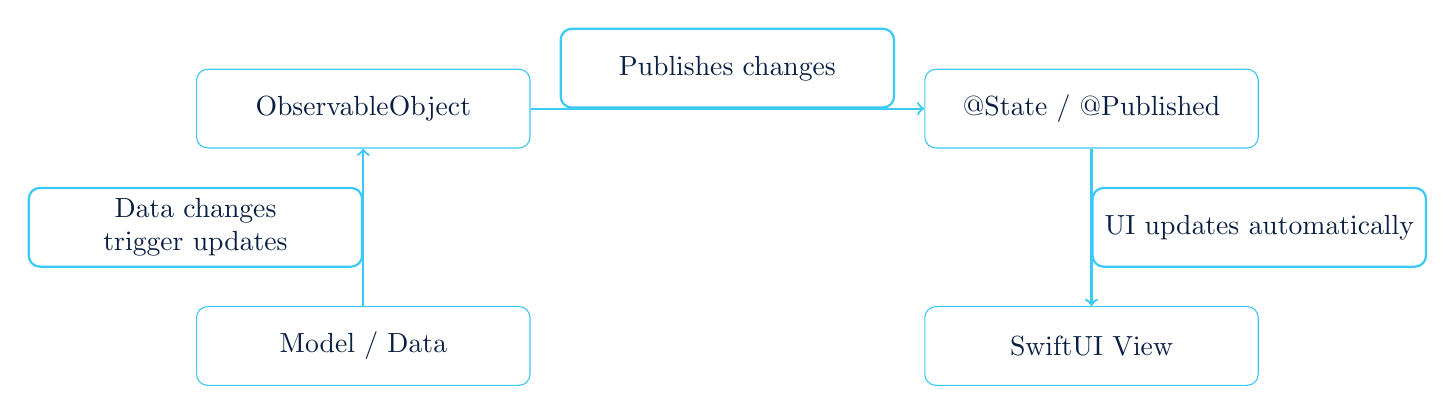
\begin{tikzpicture}[node distance=2cm, every node/.style={rectangle, rounded corners, draw=tickezyCyan, fill=white, text=tickezyNavy, text width=4cm, align=center, minimum height=1cm}]
\node (state) {@State / @Published};
\node (view) [below=2cm of state] {SwiftUI View};
\node (observable) [left=5cm of state] {ObservableObject};
\node (model) [below=2cm of observable] {Model / Data};

\draw[->, thick, tickezyCyan] (state) -- (view) node[midway,right] {UI updates automatically};
\draw[->, thick, tickezyCyan] (observable) -- (state) node[midway,above] {Publishes changes};
\draw[->, thick, tickezyCyan] (model) -- (observable) node[midway,left] {Data changes trigger updates};
\end{tikzpicture}
\caption{SwiftUI State Management Flow}
\end{figure}

\begin{tcolorbox}[speaker,title=Speaker Notes]
André: SwiftUI listens to state changes in @State or ObservableObject
and updates the UI automatically.
\end{tcolorbox}

% ---------------------------
% MVVM Architecture
% ---------------------------
\section{MVVM Architecture}

\begin{figure}[h]
\centering
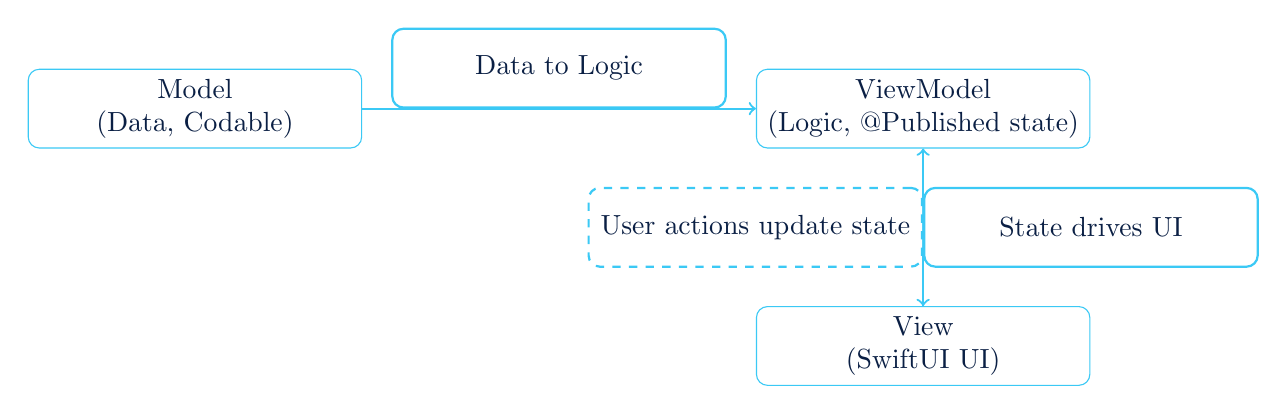
\begin{tikzpicture}[node distance=2.5cm, every node/.style={rectangle, rounded corners, draw=tickezyCyan, fill=white, text=tickezyNavy, text width=4cm, align=center, minimum height=1cm}]
\node (model) {Model \\ (Data, Codable)};
\node (viewmodel) [right=5cm of model] {ViewModel \\ (Logic, @Published state)};
\node (view) [below=2cm of viewmodel] {View \\ (SwiftUI UI)};
\draw[->, thick, tickezyCyan] (model.east) -- (viewmodel.west) node[midway,above] {Data to Logic};
\draw[->, thick, tickezyCyan] (viewmodel.south) -- (view.north) node[midway,right] {State drives UI};
\draw[->, thick, tickezyCyan, dashed] (view.north) -- (viewmodel.south) node[midway,left] {User actions update state};
\end{tikzpicture}
\caption{MVVM Architecture Flow}
\end{figure}

\begin{tcolorbox}[speaker,title=Speaker Notes]
André: MVVM separates UI from business logic,
making the app scalable and easy to maintain.
\end{tcolorbox}

% ---------------------------
% UI Wireframes with Images
% ---------------------------
\section{UI Wireframes}

\subsection{Splash Screen Wireframe}
\begin{figure}[h]
\centering
\includegraphics[width=0.6\textwidth]{tickezy_splash.png} % Replace with your splash image
\caption{Splash Screen Wireframe}
\end{figure}

\subsection{Event List Wireframe}
\begin{figure}[h]
\centering
\includegraphics[width=0.6\textwidth]{event_list.png} % Replace with your event list image
\caption{Event List Wireframe}
\end{figure}

\subsection{Ticket View Wireframe}
\begin{figure}[h]
\centering
\includegraphics[width=0.6\textwidth]{ticket_view.png} % Replace with your ticket view image
\caption{Ticket View Wireframe}
\end{figure}

% ---------------------------
% Backend Integration
% ---------------------------
\section{Backend Integration}
\begin{table}[h]
\centering
\begin{tabular}{ll}
\toprule
Feature & SwiftUI Impact \\
\midrule
Authentication & Secure login flow \\
QR Code & Digital ticket display \\
PDF Ticket & Downloadable passes \\
Email & Confirmation feedback \\
\bottomrule
\end{tabular}
\caption{Backend Features Supporting UX}
\end{table}

\begin{tcolorbox}[speaker,title=Speaker Notes]
André: Backend services exist to support
a smooth and responsive SwiftUI experience.
\end{tcolorbox}

% ---------------------------
% Challenges and Conclusion
% ---------------------------
\section{Challenges \& Lessons}
\begin{itemize}
    \item Managing asynchronous data with SwiftUI
    \item Designing reactive, state-driven UI
    \item Maintaining clean architecture while scaling features
\end{itemize}

\begin{tcolorbox}[speaker,title=Speaker Notes]
Lisa: SwiftUI taught us to think in terms of state
rather than traditional screen-based UI.
\end{tcolorbox}

\section{Conclusion}
Tickezy demonstrates the team's ability to build **scalable, real-world iOS applications** with SwiftUI.  
By combining MVVM, modern SwiftUI features, and backend support, Tickezy delivers a **smooth, intuitive, and professional user experience**.

\begin{tcolorbox}[speaker,title=Speaker Notes]
Both: Thank the audience and invite questions.
\end{tcolorbox}

\end{document}
